\chapter{Statistical models}
Now that data is cleaned and prepared, a statistical analysis consisting of data segmentation and linear regression models can be made. The purpose of the analysis is to detect which attributes affects the performance of a specific house.

\section{Linear regression}
Linear regression is a method to model the relationship between a dependent variable and one or more independent variables where the unknown model parameters are estimated from the data. \textcolor{red}{Mangler nok lidt her.} With the dependent variable $Y$ and the independent variables $x_1, \dots, x_n$, the linear regression model is formulated as
\begin{equation}
    Y_i = \beta_0 + \beta_1 x_{i,1} + \beta_2 x_{i,2} + \cdots + \beta_p x_{i,p} + \varepsilon_i, \quad \varepsilon_i ~ \mathcal{N}(0,\sigma^2), \quad i = 1,\dots, n. \label{lm}
\end{equation}
The variables $\varepsilon_i$ are errors which are assumed to be white noise while also being i.i.d (independent and identically distributed). Equation \eqref{lm} shows a multiple linear regression model as it contains more than one explanatory variable. In this section both a simple linear model and a multiple linear model has been fitted to data given in table \ref{tab: modeldata}.

\noindent As the best linear model $Y_i$ is desired, the total deviation from the data has to be as small as possible. The least squares method given as
\begin{equation}
    \text{SSE} = \sum_{i=1}^n (Y_i - (\beta_0 + \beta_1 x_{i,1} + \beta_2 x_{i,2} + \cdots  \beta_p x_{i,p}))^2 = \sum_{i=1}^n (Y_i - \Hat{Y}_i)^2
\end{equation}
is chosen for estimating the model. The parameters $\beta_j$ are optimized to minimize the sum of squared errors of prediction (SSE).

\subsection{Model assumptions}
\noindent When SSE is minimized the model needs to be validated by checking whether the underlying model assumptions are fulfilled.
\begin{enumerate} [label=\textbf{\arabic*}]
    \item Normality of residuals
    \item Variance homogenity
    \item Variance should be independent of location
    \item Linear relationship between $x_j$ and $Y$
\end{enumerate}
Chapter 7 in \cite{Stat_bog} explains the model assupmtions listed above. To summarize, a model can be checked by looking at diagnostic plots of the residuals. The first plot considered is the Residuals vs Fitted, where the residuals are expected to be randomly scattered. To test whether the residuals are normally distributed a normal quantile–quantile plot is used. Here the residuals are expected to follow a straight line. A Scale-Location plot shows normalized and weighted residuals by sample leverage where the residuals are also expected to be randomly scattered. The last diagnostic plot shows the Residuals vs Leverage which should be a straight line and there should not be any clear patterns. If these assumptions are not met, it can influence the parameter estimates and with it the significance of the parameters. In addition, a Shapiro-Wilk test is performed to check if the residuals of the models are i.i.d with $\mathcal{N}(0,\sigma^2)$. \\

\noindent The fitting of the regression models is carried out by using the method stepwise regression which updates the model in each step. In each step it is considered whether a variable is added or subtracted from the set of explanatory variables based on specific criteria. This process is called variable selection and Chapter 7 in \cite{Stat_bog2} explains how this process can be done by using either forward or backward selection. In this project a modified version of backward selection is applied. The models are used for comparing which explanatory variables influence each house. Therefore, the models are not reduced using the \texttt{R} function \texttt{step}. Instead the signifance of the parameters are investigated and then the parameters which are significant for the majority of the houses will be used in an updated linear regression model. Thus, the variable selection is done manually which can be said to be a modified form of backward selection. The level of signifance is determined by an F-test where the variables selected have a p-value below a threshold which is chosen at 0.05. \textcolor{red}{Mangler nok en ref. til det her.}\\

\noindent Both a simple linear and a multiple linear regression model will be implemented in order to detect which attributes affect the performance of a specific house. This will be done by interpreting the estimates of the relation between the different explanatory attributes and \texttt{Consumption}. As mentioned, the p-value of the estimates of the explanatory variables will be the main focus when investigating which attributes influence the performance. 

\section{Simple linear regression model}
A simple linear regression model is fitted to each house with \texttt{Consumption} as a function of \texttt{Temperature} (here denoted HC and T). Since it is expected that the temperature is the physical phenomenon with the greatest influence on the heat consumption, it is chosen as the independent variable. The models are performed by using the \texttt{lm()} function. The models will then be validated by examining whether the model assumptions in Chapter 4.1.1 are met. The simple model only includes one explanatory variable, thus a variable selection is not performed. \textcolor{red}{Begrundelse for at vi ikke transformerer data.}

\noindent Hence, the simple linear regression model applied to each house is
\begin{equation}
    Y_s = \mu + \beta_{\text{HC}}\cdot x_{\text{T}} + \varepsilon
    \label{eq: simple}
\end{equation}

\subsection{Validation}
To validate the model, different methods are used. The abovementioned model assumptions are checked and futhermore a test of normally distributed residuals is performed. If the model assumptions are fulfilled and the residuals are i.i.d with $\mathcal{N}(0,\sigma^2)$, the model is said to be valid. 

\noindent \cref{fig: simple_lm_18} and \cref{fig: fig: simple_lm_55} shows examples of the model applied on two of the houses where one does not fulfill the assumptions and a house that overall fulfill the assumptions \textcolor{red}{skal nok lige skrives lidt bedre :-))}. The top left plot in \cref{fig: simple_lm_18} clearly shows that the residuals are not randomly scattered. \textcolor{red}{Mangler noget her.}
\begin{figure}
    \centering
    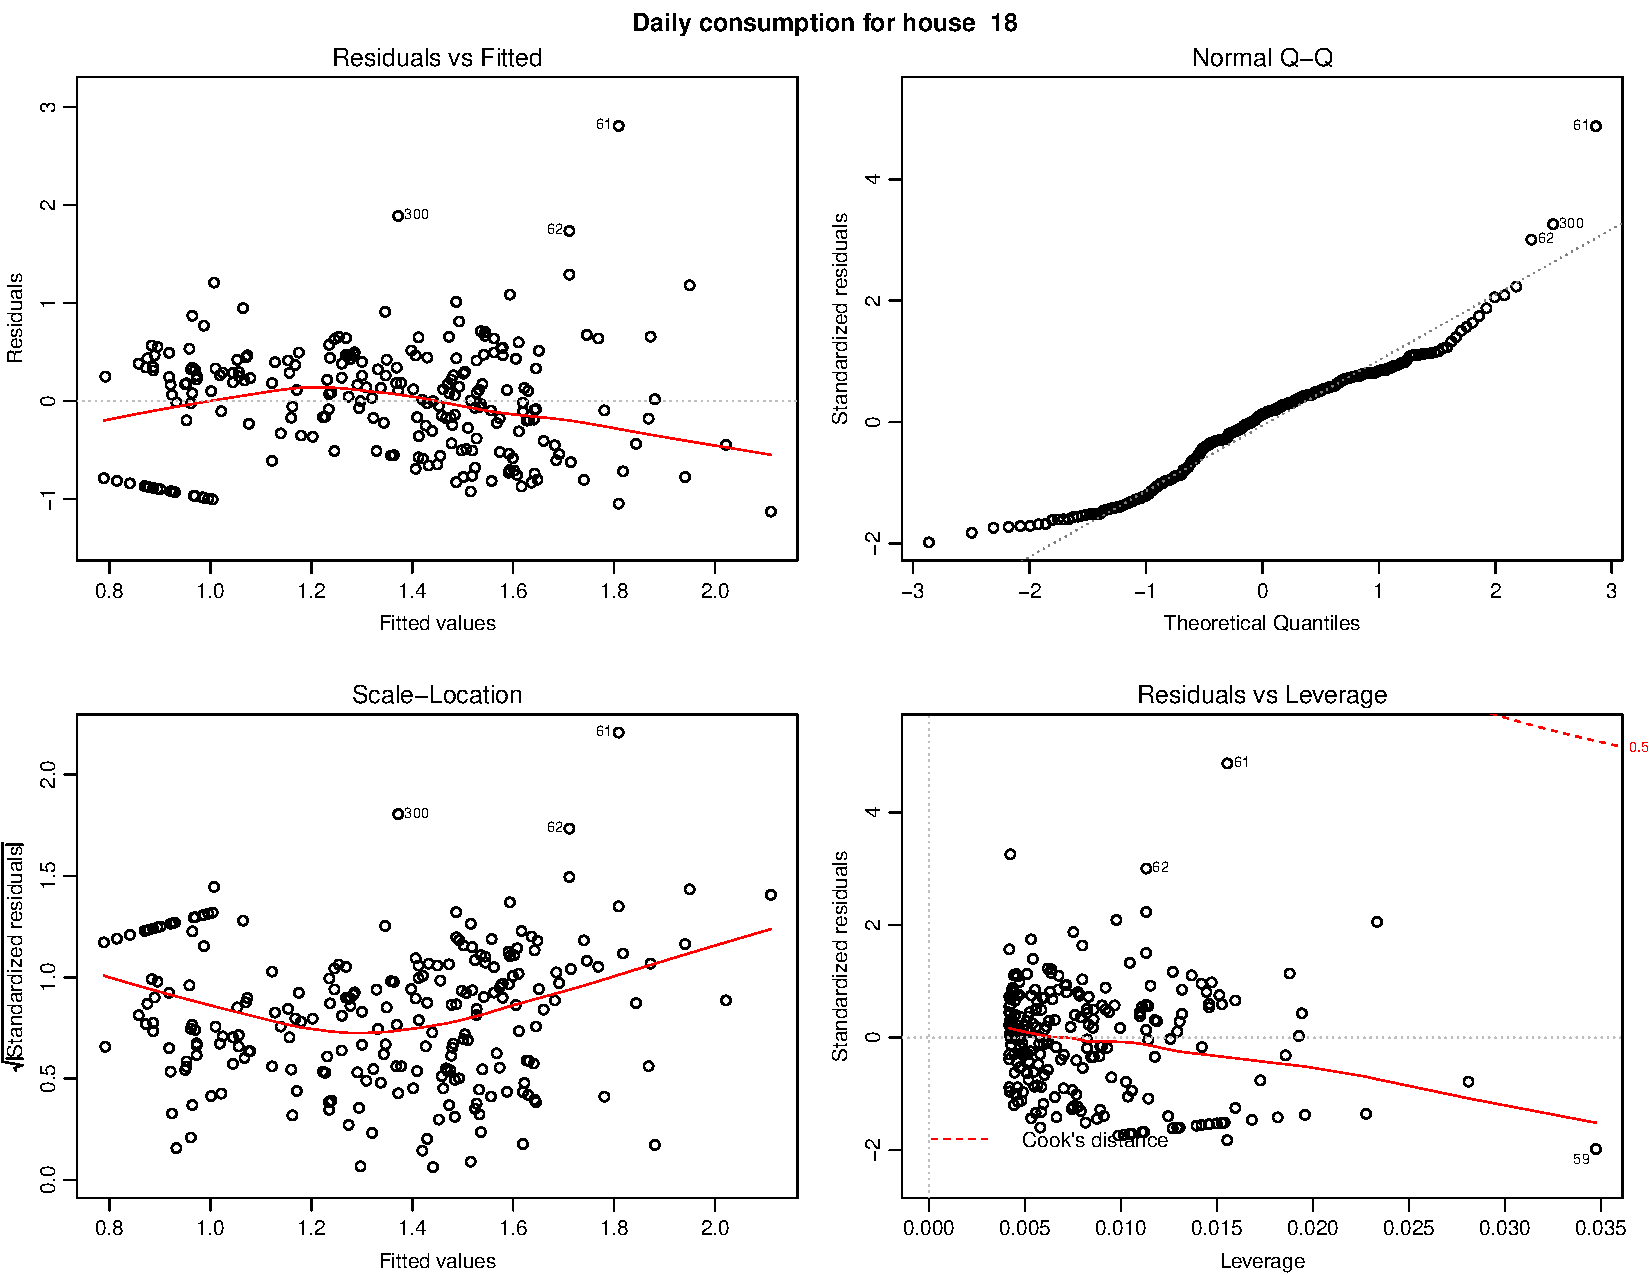
\includegraphics[width=1.\textwidth]{../../../figures/simple_lm18.pdf}
    \caption{Residual plots of house 18 based on the simple linear regression model given in \cref{eq: simple}. The model assumptions of a linear regression model are not fulfilled for this specific house}
    \label{fig: simple_lm_18}
\end{figure}

\begin{figure}
    \centering
    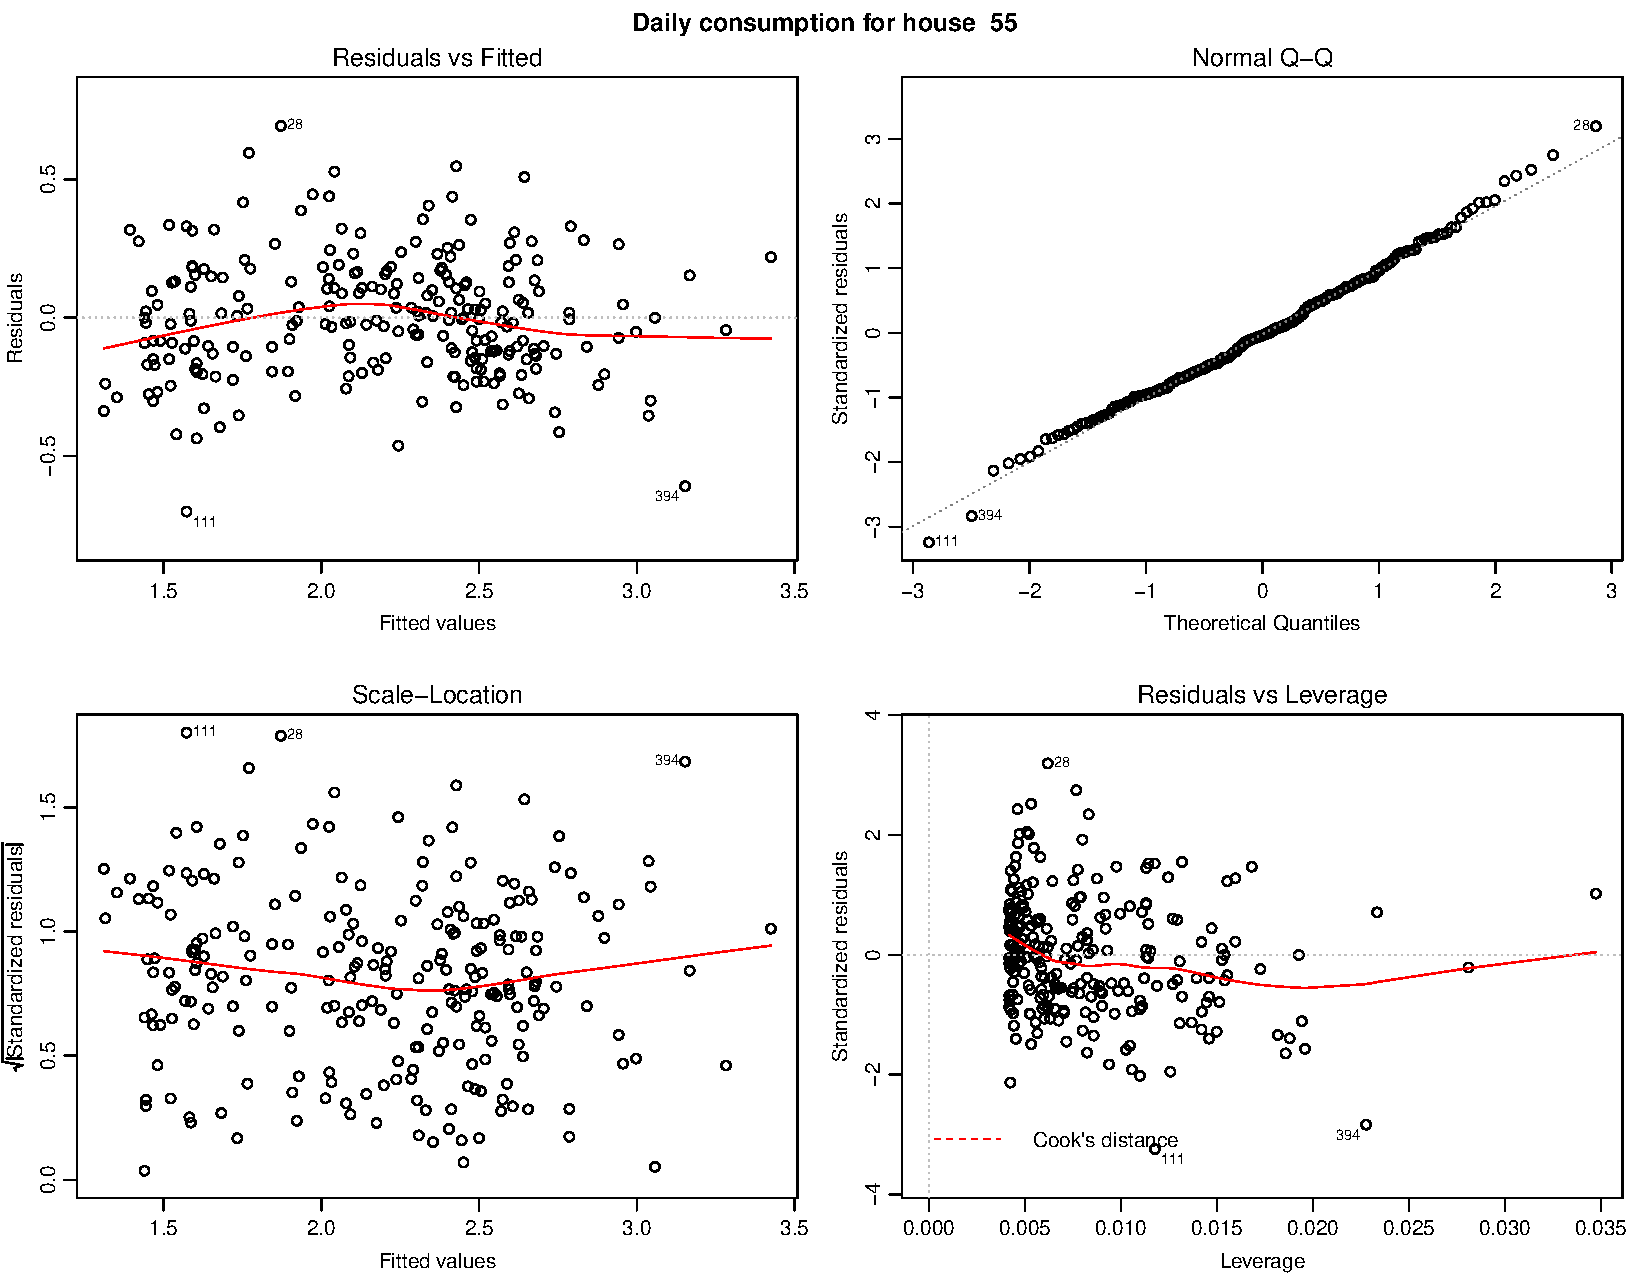
\includegraphics[width=1.\textwidth]{../../../figures/simple_lm55.pdf}
    \caption{Residual plots of house 55 based on the simple linear regression model given in \cref{eq: simple}. The model assumptions of a linear regression model are overall fulfilled}
    \label{fig: simple_lm_55}
\end{figure}

% \textcolor{blue}{Det interessante at kigge efter er de huse, hvis residuals har en mærkværdig opførsel eller den simple modellering. Som eksempel ses hus 18 i figur \ref{fig: simple_lm_18}. Det ses tydeligt, at residualerne for modellen for dette specifikke hus er gakket. Q-Q plottet ligger ikke fint langs en ret linje. Residuals vs. fitted viser en underlig opførsel, som ikke er randomly scattered.}

\subsection{Results}
\cref{tab: est_simple_lm} shows the estimates from all the simple linear regression models. 
\noindent \textcolor{blue}{Overordnet kan den simple lineære regressionsmodel ikke beskrive trenden. Den antager, at temperaturen er den eneste faktor der påvirker husenes varmeforbrug. Men ved at undersøge hvorvidt model assumptions er opfyldt, så 'failer' modellen i de fleste tilfælde. Dette tyder på, at der findes flere faktorer, der påvirker varmeforbruget, hvilket selvfølgelig er forventet.}

\section{Multiple linear regression model}
The linear regression model is extended to a multiple linear regression model as the inclusion of several independent variables is expected to improve the model. The simple model clearly showed that the heat consumption is affected by other physical factors than temperature. Hence, a full multiple linear regression model containing the attributes given in Table \ref{tab: modeldata} is performed on the model data. Since \texttt{Condition} and \texttt{PrecipitationProbability} are not normalised, they are excluded from the model. In addition, it is mentioned in Chapter 2 that the house data consists of house with observations for approximately a year and house with observations for approximately six months. Thus, the two distinct lengths of observations are modeled slighty different. There do not exist observations for winter break and spring break in the data containing the short houses. This lead to the following two multiple linear regression models: 
\textcolor{red}{Indsæt modellerne.}

\noindent The models show that the interactions between the attribute \texttt{Holiday} and the other attributes are chosen to be excluded. The reason is that \texttt{Holiday} is used to investigate how the consumption changes during holiday periods. The parameters will be denoted as follows: Intercept (I), Temperature (T), North (N), East (E), South (S), West (W), Mean Sea Level (MSL), Solar Radiation (SR), Winter Break (WB), Spring Break (SB), Autumn Break (AB), Christmas Break (CB), Weekend (WKND), the interaction between the temperature and the different wind directions (T:N, T:E, T:S, T:W). 

\subsection{Splines}
In the multiple regression model, splines will be used to model the wind direction. It does not make much sence to include the wind direction as it is in the model. It is not useful to know how significant the wind direction is, if it is not connected to the wind speed and if it is not known which directions are important. By modeling the wind direction with splines, each spline will represent a specific general direction.

Modellere wind direction
Lave en parameter om til flere vind retninger.
2. degree splines
Knots
Mellem retningerne
Giver mere mening for brugeren

\textcolor{red}{Vi vil gerne vægte vores vind i forskellige retninger i vores model, så derfor bruger vi splines til at modellere de forskellige retninger.} \\

\textcolor{red}{Tilføj billede af splines}

\subsection{Results}
\noindent When performing the two models given in \textcolor{red}{en eller anden ref til en ligning her}, without reduction, \textcolor{red}{Et eller andet} \cref{tab: lmMult_full_S}.  In addition, \cref{tab: lmMult_full_L_sum} and \cref{tab: lmMult_full_S_sum} are generated in order to determine which parameters are significant for the majority of the houses. 
\begin{table}
    \centering
    \resizebox{0.70\textheight}{!}{\begin{tabular}{l|cccccccccccccccccccc}
     \hline 
    & I & T & N & E & S & W & MSL & SR & WB & SB & AB & CB & WKND & T:N & T:E & T:S & T:W \\
    \hline 
    Sum of *** & 5 & 41 & 0 & 18 & 2 & 24 & 6 & 22 & 3 & 3 & 1 & 5 & 4 & 0 & 1 & 7 &9 \\
    Sum of ** & 6 & 1 & 1 & 9 & 5 & 12 & 4 & 10 & 6 & 2 & 0 & 2 & 0 & 1 & 1 & 9 & 9 \\
    Sum of * & 6 & 1 & 5 & 7 & 7 & 2 & 2 & 2 & 3 & 6 & 5 & 3 & 8 & 2 & 3 & 5 & 11 \\
    \hdashline
    Total of 43 & 17 & 43 & 6 & 34 & 14 & 38 & 12 & 34 & 12 & 11 & 6 & 10 & 12 & 3 & 5 & 21 & 29 \\
    \hline
\end{tabular}}
\caption{The distribution of significant parameters from the multiple linear regression model for long houses. There are 43 long houses, thus the total of the signifance of each parameter for each house is in relation to the number of long houses}
\label{tab: lmMult_full_L_sum}
\end{table}

\begin{table}
    \centering
    \resizebox{0.7\textheight}{!}{\begin{tabular}{l|cccccccccccccccccc}
     \hline 
    & I & T & N & E & S & W & MSL & SR & AB & CB & WKND & T:N & T:E & T:S & T:W \\
    \hline 
    Sum of *** & 0 & 27 & 0 & 4 & 0 & 15 & 0 & 5 & 2 & 0 & 0 & 0 & 0 & 0 & 3\\
    Sum of ** & 2 & 0 & 0 & 6 & 2 & 5 & 2 & 6 & 0 & 0 & 3 & 0 & 0 & 2 & 5 \\
    Sum of * & 2 & 0 & 1 & 8 & 4 & 4 & 4 & 4 & 2 & 5 & 2 & 1 & 1 & 3 & 9 \\
    \hdashline
    Total of 27 & 4 & 27 & 1 & 18 & 6 & 24 & 6 & 15 & 4 & 5 & 5 & 1 & 1 & 6 & 17\\
    \hline
\end{tabular}}
\caption{The distribution of significant parameters from the multiple linear regression model for short houses. As for the long houses, the total of the signifance is in relation to the number of long houses}
\label{tab: lmMult_full_S_sum}
\end{table}

\textcolor{blue}{Hvis bare én af retningerne har over halvdelen signifikant skal alle retningerne med.}

\section{Regression model for comparing houses}
\textcolor{blue}{Baseret på tabeller over signifikante parametre for både korte og lange huse, kan vi lave en general model for alle huse, der inkluderer temperaturen, splines og radiation.}

\begin{table}
    \centering
    \begin{tabular}{cccccccccccc}
     \hline
     Index & I & T & N & E & S & W & SR & T:N & T:E & T:S & T:W \\
    \hline
    1& \Plus *** & \Minus *** &  &  &  & \Plus ** &  &  &  & \Plus . & \Minus ** \\
2& \Plus *** & \Minus *** &  & \Plus ** &  & \Plus *** & \Minus *** &  &  &  & \Minus *** \\
3& \Plus *** & \Minus *** &  & \Plus *** &  & \Plus *** & \Minus *** &  &  & \Plus * & \Minus * \\
4& \Plus *** & \Minus *** & \Plus * &  & \Plus *** &  & \Minus *** &  &  &  &  \\
5& \Plus *** & \Minus *** &  & \Plus *** &  & \Plus *** & \Minus *** & \Plus * &  & \Plus *** & \Minus ** \\
7& \Plus *** & \Minus *** & \Minus ** & \Plus *** & \Minus . & \Plus ** & \Plus *** &  & \Minus ** & \Plus * & \Minus ** \\
11& \Plus *** & \Minus *** &  & \Plus *** &  & \Plus *** & \Minus *** &  &  & \Plus * &  \\
12& \Plus *** & \Minus *** &  & \Plus . &  & \Plus * &  &  &  &  &  \\
14& \Plus *** & \Minus *** &  & \Plus *** &  & \Plus *** & \Minus ** &  &  & \Plus ** &  \\
18& \Plus *** & \Minus ** &  & \Plus *** & \Minus ** & \Plus ** & \Plus . &  &  & \Plus *** & \Minus *** \\
21& \Plus *** & \Minus *** &  & \Plus * &  & \Plus *** &  &  &  &  & \Minus *** \\
22& \Plus *** & \Minus *** &  &  & \Plus *** & \Plus ** & \Minus *** &  &  &  & \Minus * \\
23& \Plus *** & \Minus *** & \Minus . & \Plus * &  & \Plus *** & \Minus *** &  &  & \Plus *** & \Minus *** \\
28& \Plus *** & \Minus *** &  & \Plus * & \Plus . &  & \Minus ** &  &  &  &  \\
29& \Plus *** & \Minus *** &  & \Plus *** &  & \Plus *** & \Minus ** & \Plus * &  & \Plus ** & \Minus *** \\
30& \Plus *** & \Minus *** &  & \Plus * & \Plus . & \Plus *** & \Minus *** &  &  &  & \Minus * \\
31& \Plus *** & \Minus *** &  & \Plus *** &  & \Plus *** & \Minus *** & \Plus ** &  & \Plus *** & \Minus *** \\
32& \Plus *** & \Minus ** &  &  & \Plus . & \Plus ** &  &  & \Plus . &  & \Minus . \\
33& \Plus *** & \Minus *** &  & \Plus *** & \Plus ** & \Plus *** & \Minus *** &  &  &  & \Minus ** \\
34& \Plus *** & \Minus *** &  & \Plus *** & \Plus . & \Plus *** & \Minus ** &  &  & \Plus . & \Minus ** \\
36& \Plus *** & \Minus *** &  & \Plus *** &  & \Plus *** & \Minus *** &  &  & \Plus ** &  \\
37& \Plus *** & \Minus *** &  & \Plus *** & \Plus ** & \Plus ** & \Minus *** &  &  &  &  \\
38& \Plus *** & \Minus *** &  & \Plus * &  & \Plus *** & \Minus *** &  &  &  & \Minus *** \\
40& \Plus *** & \Minus *** &  & \Plus . & \Plus ** & \Plus ** & \Minus *** &  & \Plus . & \Plus * & \Minus * \\
41& \Plus *** & \Minus *** &  & \Plus *** & \Plus . & \Plus *** &  &  & \Plus . & \Plus . & \Minus . \\
42& \Plus *** & \Minus *** &  & \Plus *** &  & \Plus *** & \Minus *** &  &  &  & \Minus * \\
44& \Plus *** & \Minus *** & \Minus * &  &  &  & \Minus ** &  &  & \Plus * &  \\
45& \Plus *** & \Minus *** &  &  & \Plus * & \Plus *** & \Minus * &  & \Plus * & \Plus * & \Minus *** \\
46& \Plus *** & \Minus *** &  & \Plus * & \Plus * & \Plus *** & \Minus ** &  &  &  & \Minus ** \\
47& \Plus *** & \Minus *** &  & \Plus ** &  & \Plus *** & \Minus ** &  & \Minus ** &  & \Minus *** \\
48& \Plus *** & \Minus *** &  & \Plus ** & \Plus * & \Plus *** & \Minus ** &  &  &  & \Minus ** \\
49& \Plus *** & \Minus *** &  &  &  &  & \Minus ** &  &  &  &  \\
50& \Plus *** & \Minus *** & \Minus . & \Plus *** & \Minus * & \Plus ** & \Minus *** & \Plus . &  & \Plus *** & \Minus . \\
52& \Plus *** & \Minus *** & \Minus . &  & \Minus ** & \Minus . & \Minus *** &  &  & \Plus *** &  \\
54& \Plus *** & \Minus *** &  & \Plus ** &  & \Plus ** & \Minus *** &  &  & \Plus * & \Minus * \\
55& \Plus *** & \Minus *** &  & \Plus * & \Plus . & \Plus *** & \Minus *** &  &  & \Plus ** & \Minus * \\
56& \Plus *** & \Minus *** &  & \Plus ** &  & \Plus *** & \Minus *** &  &  & \Plus ** & \Minus * \\
57& \Plus *** & \Minus *** &  & \Plus *** &  & \Plus *** &  &  &  &  & \Minus ** \\
58& \Plus *** & \Minus *** & \Minus . & \Plus . &  & \Plus *** & \Minus *** & \Plus * &  & \Plus *** & \Minus ** \\
61& \Plus *** & \Minus *** &  & \Plus * & \Plus . & \Plus * &  & \Minus . &  & \Minus . &  \\
64& \Plus *** & \Minus *** & \Minus * & \Plus *** &  & \Plus *** & \Minus *** &  & \Minus . & \Plus ** & \Minus ** \\
65& \Plus *** & \Minus *** &  & \Plus * &  & \Plus *** & \Minus *** &  &  & \Plus * & \Minus ** \\
66& \Plus *** & \Minus *** & \Plus . & \Plus *** & \Plus ** & \Plus *** & \Minus *** &  &  & \Plus ** & \Minus ** \\
    \hline
    \end{tabular}
    \caption{Significance of parameters for 'long' houses. \textcolor{red}{Punktum betyder, at det er mellem 5 og 10\%}}
    \label{lmMult_gen_L}
\end{table}

\begin{table}[H]
    \centering
    \begin{tabular}{cccccccccccc}
     \hline
     Index & I & T & N & E & S & W & SR & T:N & T:E & T:S & T:W \\
    \hline
6& \Plus *** & \Minus *** &  & \Plus . &  & \Plus ** & \Minus * &  &  &  &  \\
8& \Plus *** & \Minus *** &  & \Plus * &  & \Plus *** & \Minus * &  &  & \Plus * & \Minus . \\
9& \Plus *** & \Minus *** & \Minus . &  &  & \Plus * & \Minus *** & \Plus * &  & \Plus * & \Minus ** \\
10& \Plus *** & \Minus *** &  & \Plus *** &  & \Plus ** & \Minus ** &  &  &  & \Minus . \\
13& \Plus *** & \Minus *** &  & \Plus . &  & \Plus ** & \Minus . & \Plus . &  & \Plus ** & \Minus ** \\
15& \Plus *** & \Minus *** &  & \Plus ** &  & \Plus ** &  &  &  &  &  \\
16& \Plus *** & \Minus *** &  & \Plus . &  & \Plus *** & \Minus * &  &  &  & \Minus ** \\
17& \Plus *** & \Minus *** &  & \Plus * & \Plus *** & \Plus *** & \Minus ** &  &  &  & \Minus *** \\
19& \Plus *** & \Minus *** &  & \Plus * & \Minus . &  &  & \Plus . &  & \Plus ** &  \\
20& \Plus *** & \Minus *** &  &  & \Plus * &  &  &  &  &  &  \\
24& \Plus *** & \Minus *** &  & \Plus * &  & \Plus *** &  &  &  &  & \Minus *** \\
25& \Plus *** & \Minus *** &  & \Plus ** &  & \Plus *** &  &  &  & \Plus * & \Minus * \\
26& \Plus *** & \Minus *** &  &  &  & \Plus *** & \Minus * & \Plus . &  & \Plus * & \Minus * \\
27& \Plus *** & \Minus *** &  & \Plus . & \Plus ** & \Plus ** &  &  &  &  & \Minus * \\
35& \Plus *** & \Minus *** &  & \Plus ** & \Plus . & \Plus *** & \Minus ** &  &  &  & \Minus ** \\
39& \Plus *** & \Minus *** &  &  &  & \Plus * & \Minus * &  &  & \Plus . &  \\
43& \Plus *** & \Minus *** &  & \Plus ** & \Plus . & \Plus *** & \Minus ** &  &  &  & \Minus ** \\
51& \Plus *** & \Minus *** &  &  & \Plus . & \Plus *** & \Minus ** &  &  & \Plus * & \Minus ** \\
53& \Plus *** & \Minus *** &  & \Plus * &  & \Plus * &  &  &  &  & \Minus . \\
59& \Plus *** & \Minus *** & \Minus * & \Plus ** & \Plus * & \Plus *** & \Minus * & \Plus * &  & \Plus * & \Minus . \\
60& \Plus *** & \Minus *** & \Minus * & \Plus ** &  & \Plus *** & \Minus *** & \Plus ** &  & \Plus ** & \Minus *** \\
62& \Plus *** & \Minus *** &  &  &  & \Plus * & \Minus * &  &  &  &  \\
63& \Plus *** & \Minus *** &  & \Plus * &  &  &  &  &  & \Plus . &  \\
67& \Plus *** & \Minus *** &  & \Plus *** &  & \Plus *** & \Minus *** &  & \Minus * & \Plus . & \Minus ** \\
68& \Plus *** & \Minus *** &  &  &  & \Plus * & \Minus *** &  &  & \Plus * & \Minus * \\
69& \Plus *** & \Minus *** &  &  &  & \Plus ** & \Minus * &  & \Plus * &  &  \\
70& \Plus *** & \Minus *** &  & \Plus . &  & \Plus *** & \Minus *** &  &  &  & \Minus ** \\
    \hline
    \end{tabular}
    \caption{Significance of parameters for 'short' houses. \textcolor{red}{Punktum betyder, at det er mellem 5 og 10\%}}
    \label{lmMult_gen_S}
\end{table}

\subsection{Validation}

\subsection{Results}

\section{Comparison}
